\documentclass[11pt]{beamer}
\usepackage[utf8]{inputenc}
\usepackage[T1]{fontenc}
\usetheme{Pittsburgh}
\usepackage{booktabs}

\usepackage{graphicx,epstopdf,float}
\usepackage{latexsym,amsmath,amssymb,amsfonts,dsfont} 	\usepackage{multicol}[1999/05/25]					  	\usepackage{subfigure}								  	
\usepackage{hyperref}
\usepackage{color}						
\newcommand{\red}{\textcolor{red}}
\newcommand{\white}{\textcolor{white}}
\newcommand{\blue}{\textcolor{}}

\newcommand*\Laplace{\mathop{}\!\mathbin\bigtriangleup}
\begin{document}
	
	\begin{frame}
		\begin{figure}
			\centering
			\includegraphics[width=2 cm]{fig/PUCV}
		\end{figure}
		\begin{center}
			\large{ \textbf{Modelación Matemática y Simulación Computacional de un Problema Multi-Escala: Aplicación a Tejidos Cardíacos}}			
		\end{center}
		\begin{center}
			\normalsize{Felipe Galarce Marin} \\[0.2 cm]
			\begin{small}	
							
			Profesor Guía: Joaquín Mura\\
			Profesor Co-referente: Cristobal Bertoglio \\
			Pontificia Universidad Católica de Valparaíso
			\end{small}
		\end{center}
	\end{frame}

	\begin{frame}[t]
		\vspace*{0.5 cm} \textbf{Fundamentos} - Anatomía y Electrofisiología Cardíaca \\
		\color{brown}\rule{\linewidth}{4pt} \\ [0.5 cm]
		\begin{columns}[T] % align columns
			\begin{column}{.48\textwidth}
				\begin{figure}
					\centering
					\includegraphics[height= 4.5 cm]{fig/fundamentals-corazon}
				\end{figure}
			\end{column}%
			\hfill%
			\begin{column}{.6\textwidth}
				\begin{itemize}
					\item El corazón como una bomba:
					\begin{itemize}
						\item Auriculas
						\item Ventriculos
						\item Valvulas
					\end{itemize}						
					\item Pared ventriculuar gruesa (Hearth Wall)
					\begin{itemize}
						\item Endocardio
						\item Miocardio
						\item Pericardio
					\end{itemize}
					\item Pared auricular delgada.					
				\end{itemize}
			\end{column}%
		\end{columns}		
	\end{frame}
	
	\begin{frame}[t]
		\vspace*{0.5 cm} \textbf{Fundamentos} - Anatomía y Electrofisiología Cardíaca \\
		\color{brown}\rule{\linewidth}{4pt} \\ [0.5 cm]
		\begin{columns}[T] % align columns
			\begin{column}{.48\textwidth}
				\begin{figure}[H]
					\centering			
					\includegraphics[height= 3.5 cm]{fig/fundamentals-sistema_de_conduccion}
				\end{figure}
				
			\end{column}%
			\hfill%
			\begin{column}{.48\textwidth}
				\begin{itemize}
					\item Propagación del Potencial Electrico.
					\begin{itemize}
						\item Autopolarización en SAN.
						\item Autopolarización en SAN.
						\item Autopolarización en SAN.												
					\end{itemize}
				\end{itemize}
			\end{column}%
		\end{columns}
	\end{frame}

	
	\begin{frame}[t]
		\vspace*{0.5 cm} \textbf{Fundamentos} - Anatomía y Electrofisiología Cardíaca \\
		\color{brown}\rule{\linewidth}{4pt} \\ [0.5 cm]
		\begin{columns}[T] % align columns
			\begin{column}{.48\textwidth}
				\begin{figure}
				\centering
				\includegraphics[height=6.3 cm]{fig/Cardiac_Muscle}
				\end{figure}

			\end{column}%
			\hfill%
			\begin{column}{.48\textwidth}
				\begin{itemize}
					\item Miocitos.
					\item Gap junctions.
					\item Colageno.
					\item Problema multi-escala.
					\item PONER CUANTO MIDEN NORMALMENTE \\[0.5 cm]
					\includegraphics[height=2.5 cm]{fig/myocitos_foto}
				\end{itemize}
			\end{column}%
		\end{columns}	
	\end{frame}
	
	\begin{frame}[t]
		\vspace*{0.5 cm} \textbf{Fundamentos} - Anatomía y Electrofisiología Cardíaca \\
		\color{brown}\rule{\linewidth}{4pt} \\ [0.5 cm]
		\begin{columns}[T] % align columns
			\begin{column}{.48\textwidth}
				\begin{figure}[H]
					\centering
					\includegraphics[height = 5 cm]{fig/fundamentals-direccionmiocitos}
				\end{figure}			
				\end{column}%
				\hfill%
				\begin{column}{.48\textwidth}
					\begin{itemize}
						\item Tres direcciónes.
						\item Gap Junctions.
						\item Anisotropía.
						\item Orientación de las fibras cardíacas.
					\end{itemize}
				\end{column}%
			\end{columns}	
		
	\end{frame}

	

	\begin{frame}[t]
		\vspace*{0.5 cm} \textbf{Fundamentos} - Fibrosis
		\color{brown}\rule{\linewidth}{4pt} \\ [0.2 cm]
		\begin{itemize}
			\item Definicion
			\item Importancia de su estudio
			\begin{itemize}
				\item[-] Fibrosis  $\rightarrow$ Fibrilación Ventricular $\rightarrow$ Paro Cardíaco (sudden cardiac arrest)
				\item[-] Fibrosis $\rightarrow$ Propagación del Potencial Eléctrico en el tejido cardíaco \cite{TenTusscher2007Europace}
				COMPLEMENTAR CON CITAS Y DATOS DE INFORME ACTUALIZADO
			\end{itemize}
			\item Tipos de Fibrosis
		\end{itemize}
		
		\begin{figure}
			\centering
			\includegraphics[width= 10 cm]{fig/tipos_de_fibrosis}
		\end{figure}
	\end{frame}

	\begin{frame}[t]
		\vspace*{0.5 cm} \textbf{Modelación} - Ecuacion de Monodominio
		\color{brown}\rule{\linewidth}{4pt} \\ [0.2 cm]
		\begin{itemize}
			\item Tejido fibrado conductor (diffusion)
			\item Potencial de acción (reacción) \\[0.5 cm]
		\end{itemize}
		\begin{equation*}			
		\color{black} \frac{\partial \phi}{\partial t} - \color{brown} \underbrace{\nabla \cdot (D \nabla \phi)}_{\text{Difusión}} \color{black} = \color{blue} \underbrace{I_{ion} (\phi, \vec{r})}_{\text{Reacción}}
		\end{equation*}
		\begin{figure}
			\centering
			\includegraphics[height = 3.1cm]{fig/esquema_membrana}
			\includegraphics[height = 3.1 cm]{"fig/AP real"}
		\end{figure}
		
	\end{frame}
\begin{frame}[t]
	\vspace*{0.5 cm} \textbf{Modelación} - Término de Reacción: modelo de FitzHugh–Nagumo		
	\color{brown}\rule{\linewidth}{4pt} \\ [0.2 cm]
	
	\begin{itemize}
		\item FitzHugh–Nagumo \\
		\begin{align*}
			\color{blue}
			I_{ion}(\phi, w) &= c_1 \phi (\phi - \alpha)(1 - \phi) - c_2 w \\ 
			\dfrac{\partial w}{\partial t} &= c_2 (\phi - wd) \nonumber 
		\end{align*}		
	\begin{itemize}
		\item Una variable y 4 parámetros modelan respuesta célular. 
		\item Reducido costo computacional.
		\item No reprocude forma del potencial de acción ni periodo refractorio.
		\item Frente de onda con forma poco realista.
		\item Resultados muy aproximados, y válido solo a escala macroscópica.
	\end{itemize}		
	\end{itemize}
\end{frame}	

\begin{frame}[t]
	\vspace*{0.5 cm} \textbf{Modelación} - Término de Reacción: modelo Minimal	
	\color{brown}\rule{\linewidth}{4pt} \\ [0.2 cm]
	\begin{itemize}
		\item Modelo Minimal \\[0.2 cm]
		\centering	$ \color{blue} I_{ion}(\phi, r, w, s) \color{black} = - (J_{fi} + J_{so} + J_{si}) $ \\[.1 cm]

		\flushleft
		$\partial_t r = (1 - H(\phi - \theta_v))(r_\infty - r)/\tau_{v}^- - H(\phi - \theta_v)r/\tau_v^+ $ \\
		$\partial_t w = (1 - H(\phi - \theta_w))(w_\infty - w)/\tau_{w}^- - H(\phi - \theta_w)w/\tau_w^+ $ \\
		$\partial_t s = ((1 + tanh(k_s(\phi - \phi_s)))/2 - s)/\tau_s $ \\[.1 cm]

		\begin{itemize}
			\item Tres variables y 28 parámetros modelan respuesta celular.
			\item Se considera la diferencia de potencial producida por el paso de iones a través de canales ($J_{fi}$) y a través de la membrana fosfolipídica ($J_{so}$ y $J_{si}$).
			\item Reproduce de forma realista forma y propiedades del potencial de acción.
			\item Resultados válidos en meso-escala y macro-escala.
		\end{itemize}		
	\end{itemize}
\end{frame}

\begin{frame}[t]
	\vspace*{0.5 cm} \textbf{Simulación} - Modelo de FitzHugh–Nagumo.
	\color{brown}\rule{\linewidth}{4pt} \\ [0.2 cm]
	
	\begin{itemize}
		\item Se desprecia difusión (una sola célula).
		\item Discretización temporal semi-implicita. $\Delta t = 1~[ms]$.
		\item Condiciones iniciales:  $\phi(0) = 0.2$ y $r(0) = 0$.
	\end{itemize}
	
  \begin{figure}[H]
  	\centering 
  	\includegraphics[height = 5 cm]{fig/EX1-FHN_single_cell.eps}
  \end{figure}
\end{frame}

\begin{frame}[t]
\vspace*{0.5 cm} \textbf{Simulación} - Modelo Minimal.
\color{brown}\rule{\linewidth}{4pt} \\ [0.2 cm]

\begin{itemize}
	\item Se desprecia difusión (una sola célula).
	\item Discretización temporal semi-implicita. $\Delta t = 0.1~[ms]$.
	\item Condiciones iniciales: $\phi = 0$, $r = 1$, $w = 1$ y $s = 0$.
\end{itemize}

	\begin{figure}[!htbp]
		\centering
		\subfigure[Celula epicardial.]{
			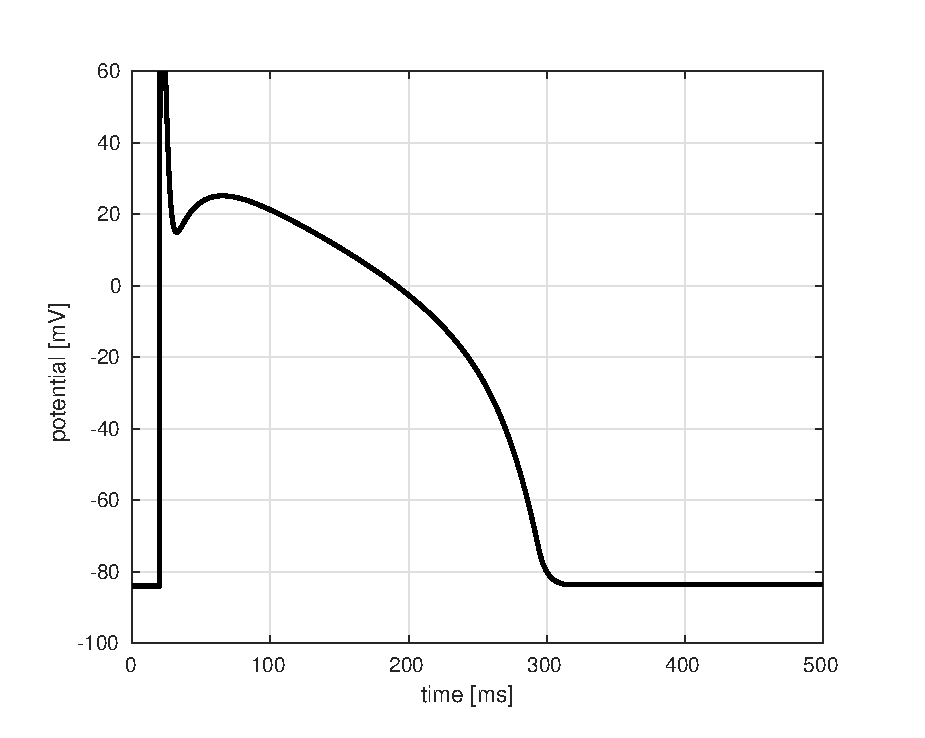
\includegraphics[width = 4 cm]{fig/ex1_min_epi}}
		\subfigure[Célula auricular.]{
			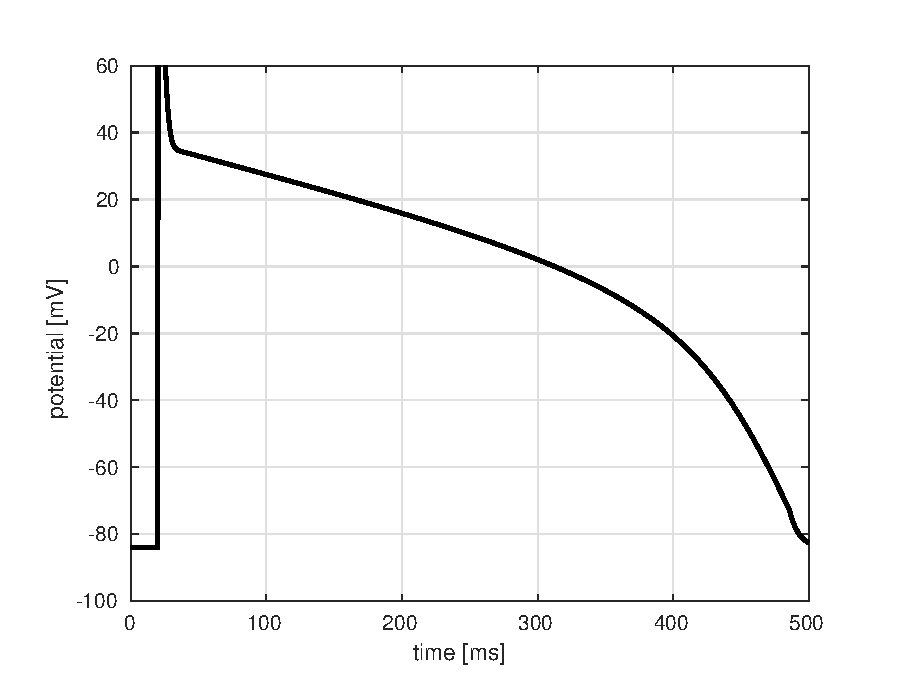
\includegraphics[width = 4 cm]{fig/ex1_min_mid}}
	\end{figure}	
\end{frame}

\begin{frame}[t]
	\vspace*{0.5 cm} \textbf{Problema Multi-Escala} - Homogeneización
	\color{brown}\rule{\linewidth}{4pt} \\ [0.2 cm]
	
	\begin{columns}[T] % align columns
		\begin{column}{.8\textwidth}
		\begin{itemize}
			\item Dos escalas de interes: a nivel de celula (meso-escala) y a nivel de tejido (macro-escala).
			\item A nivel celular, la fibrosis aparece como incustraciones de colageno alrededor de las fibras musculares. En consecuencia, resulta natural la utilización de algunos resultados de la teoría de homogeneización para materiales fibrados.

		\end{itemize}

		\end{column}%
		\hfill%
		\begin{column}{.3\textwidth}
			\begin{figure}[H]
				\centering 
				\includegraphics[height = 3.6 cm]{fig/miocitos_cardiacos}
			\end{figure}
		\end{column}%
	\end{columns}


\end{frame}

\end{document}